\section{Encerramento}
\begin{wrapfigure}{l}{0.28\textwidth}

\begin{center}
  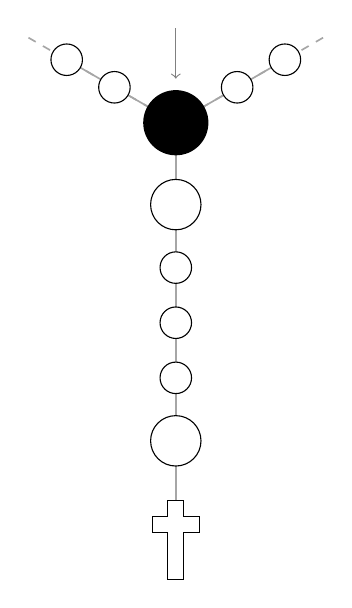
\begin{tikzpicture}[scale=0.8]

    \coordinate (center) at (0,0);
    \coordinate (cross-origin) at (0,-6);

% linha da cruz
\draw[gray!70, line width=0.6pt] (cross-origin) -- (center);

\draw[fill=white] (0,-1.3) circle (0.4) ++ (0,-1) circle (0.25)  ++ (0, -0.875) circle (0.25) ++ (0, -0.875) circle (0.25) ++ (0, -1) circle (0.4);

% contas maiores
% \draw[fill=white] (0,-5) circle (0.4);

% cruz
\draw[black] (cross-origin) -- ++(0.125, 0) -- ++(0,-.25) -- ++(.25,0) -- ++(0,-.25) -- ++ (-.25,0) -- ++(0, -.75) -- ++(-.25,0) -- ++ (0,.75) --++ (-.25,0) -- ++ (0,.25) -- ++ (.25,0) -- ++ (0,.25) -- (cross-origin);

% linha com ângulo
\draw[gray!70, line width=0.6pt, dashed] ({150}:2.7) -- (center);
\draw[gray!70, line width=0.6pt] ({150}:2) -- (center);

\draw[fill=white] ({150}:1.125) circle (0.25);
\draw[fill=white] ({150}:2) circle (0.25);

% linha com ângulo
\draw[gray!70, line width=0.6pt, dashed] ({30}:2.7) -- (center);
\draw[gray!70, line width=0.6pt] ({30}:2) -- (center);

\draw[fill=white] ({30}:1.125) circle (0.25);
\draw[fill=white] ({30}:2) circle (0.25);

% círculo central
\draw[fill=black, thick] (center) circle (0.5);
\draw[gray, <-] (0,.7) --  (0, 1.5);


  \end{tikzpicture}
\end{center}

\end{wrapfigure}

Eu Vos saúdo, Maria, Filha bem-amada do Eterno Pai, Mãe admirável do Filho, Esposa mui fiel do Espírito Santo, templo augusto da Santíssima Trindade; eu Vos saúdo soberana Rainha, a quem tudo está submisso no Céu e na Terra; eu Vos saúdo, seguro refúgio dos pecadores, nossa Senhora da Misericórdia, que jamais repeliste pessoa alguma. Pecador que sou, me prostro aos Vossos pés, e Vos peço de me obter de Jesus, Vosso amado filho, a contrição e o perdão de todos os meus pecados, e a divina sabedoria. Eu me consagro todo a Vós, com tudo o que possuo. Eu Vos tomo, hoje, por minha Mãe e Senhora. Tratai-me, pois, como o último de Vossos filhos e o mais obediente de Vossos escravos. Atendei, minha Rainha, atendei aos suspiros de um coração que deseja amar-Vos e servi-Vos fielmente. Que ninguém diga que, entre todos que a Vós recorreram, seja eu o primeiro desamparado. Ó minha esperança, Ó minha vida, Ó minha fiel e imaculada Virgem Maria defendei-me, nutri-me, escutai-me, instruí-me, guardai-me. Assim seja. \textbf{Salve-Rainha}...

\subsection{Orações reparadoras reveladas pelo Anjo na aparição em Fátima, Portugal,
em 1917:}

Santíssima Trindade, Pai, Filho e Espírito Santo, adoro-Vos profundamente e ofereço-Vos o preciosíssimo Corpo, Sangue, Alma e Divindade de Jesus Cristo, presente em todos os sacrários da Terra, em reparação dos ultrajes, sacrilégios e indiferenças com que Ele mesmo é ofendido. E pelos méritos infinitos do Seu Santíssimo Coração e do Coração Imaculado de Maria, peço-Vos a conversão dos pobres pecadores.

Meu Deus, eu creio, adoro, espero e amo-Vos. Peço-Vos perdão para os que não creem, não adoram, não esperam e não Vos amam. †$^{\ref{sinal-da-cruz}}$

\newpage
